\begin{figure*}[!htbp]
    \centering
    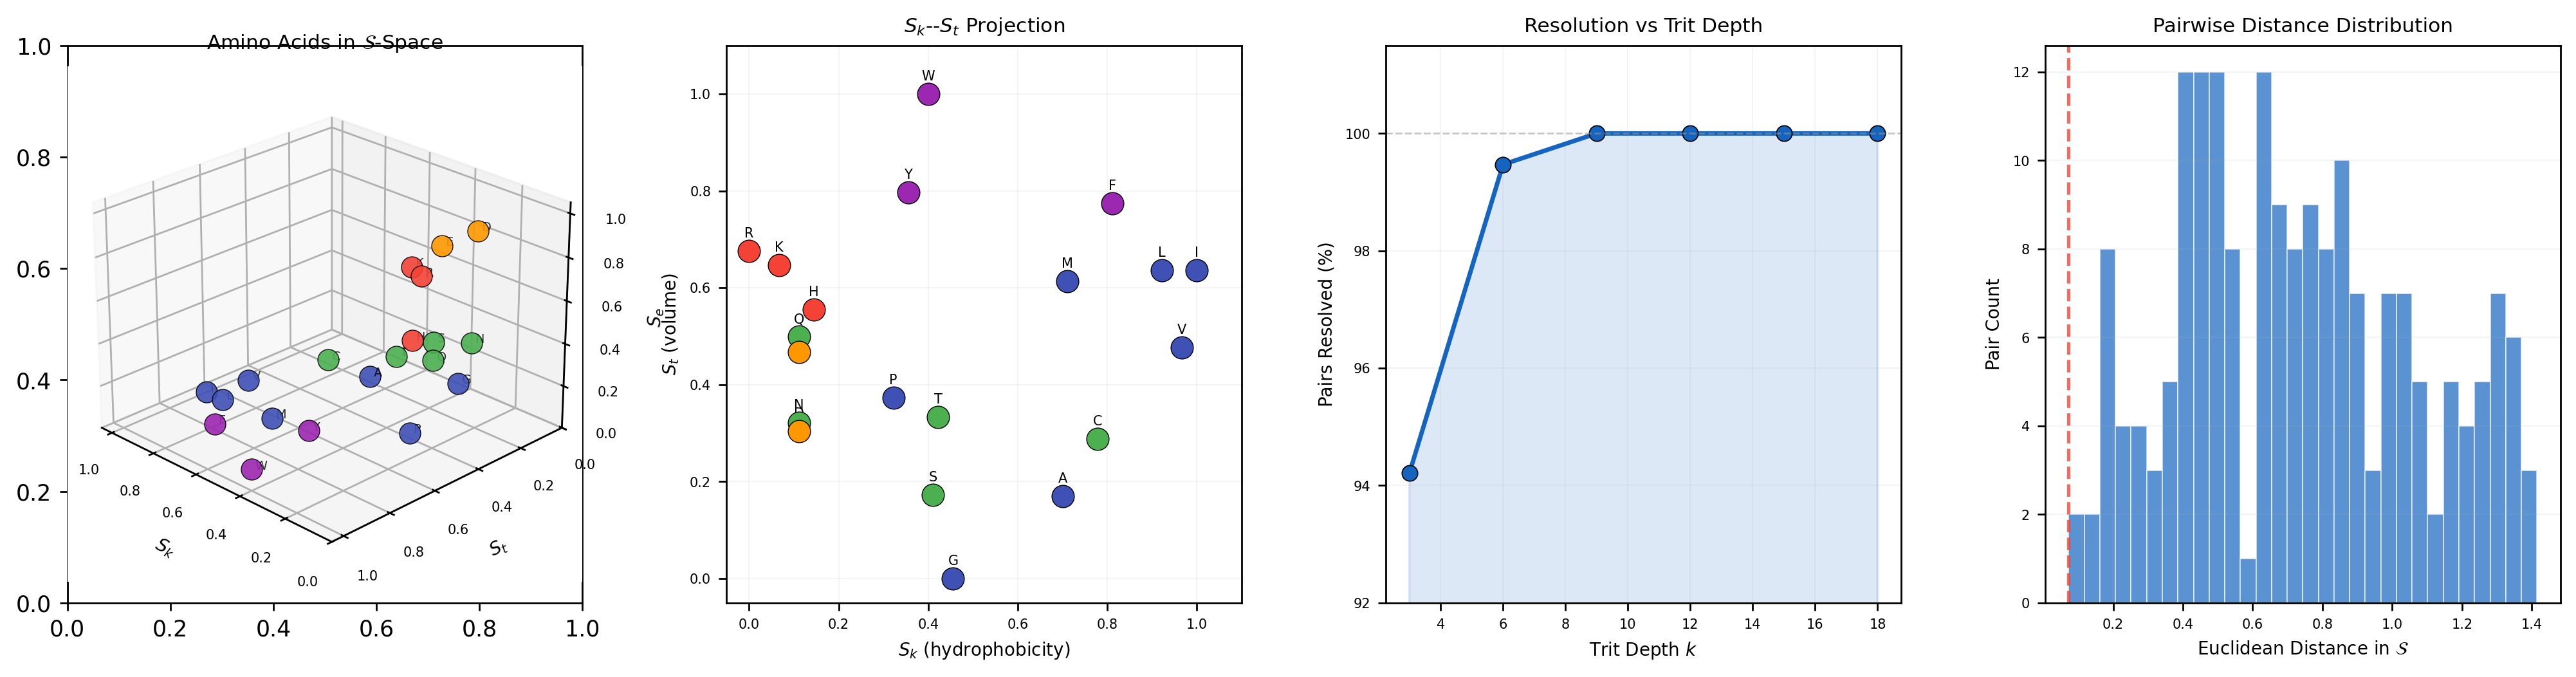
\includegraphics[width=\textwidth]{figures/panel_1_amino_acid_sentropy.png}
    \caption{\textbf{Amino Acid S-Entropy Encoding and Resolution.}
    (\textbf{A})~All 20 standard amino acids embedded in three-dimensional S-entropy space $\mathcal{S} = [0,1]^3$ with axes $S_k$ (hydrophobicity), $S_t$ (van der Waals volume), $S_e$ (electrostatic index). Points are coloured by physicochemical class: nonpolar (blue), polar (green), aromatic (purple), positively charged (red), negatively charged (orange). Charged residues cluster in the high-$S_e$ region ($S_e = 0.5$--$1.0$); nonpolar residues occupy the $S_e = 0$ plane with high $S_k$; aromatics span intermediate $S_k$ with high $S_t$ reflecting their large side-chain volumes.
    (\textbf{B})~Two-dimensional $S_k$--$S_t$ projection. Nonpolar residues (I, V, L, F, M, A) form a high-$S_k$ cluster. Glycine occupies the origin of $S_t$ (minimal volume). Tryptophan reaches $S_t = 1.0$ (largest side chain). The projection reveals a continuous gradient from small hydrophobic (Ala, $S_k = 0.70$, $S_t = 0.17$) to large aromatic (Trp, $S_k = 0.40$, $S_t = 1.00$).
    (\textbf{C})~Resolution curve: percentage of 190 pairwise amino acid combinations uniquely resolved as a function of ternary trit depth $k$. At $k = 3$, 94.2\% of pairs are resolved (12 unique addresses). At $k = 6$, 99.5\% (19 unique). Full resolution (100\%, all 20 unique) is achieved at $k = 9$, corresponding to cell width $3^{-3} \approx 0.037$ per dimension.
    (\textbf{D})~Distribution of all 190 pairwise Euclidean distances in $\mathcal{S}$-space. The minimum distance (red dashed line) is 0.073 (Lys--Arg), confirming that even the closest pair exceeds the $k = 9$ cell diagonal ($\sqrt{3} \times 3^{-3} = 0.064$). The mean distance is 0.729, with a right-skewed distribution reflecting the separation between charged and nonpolar classes.}
    \label{fig:amino_acid_sentropy}
\end{figure*}

\begin{figure*}[!htbp]
    \centering
    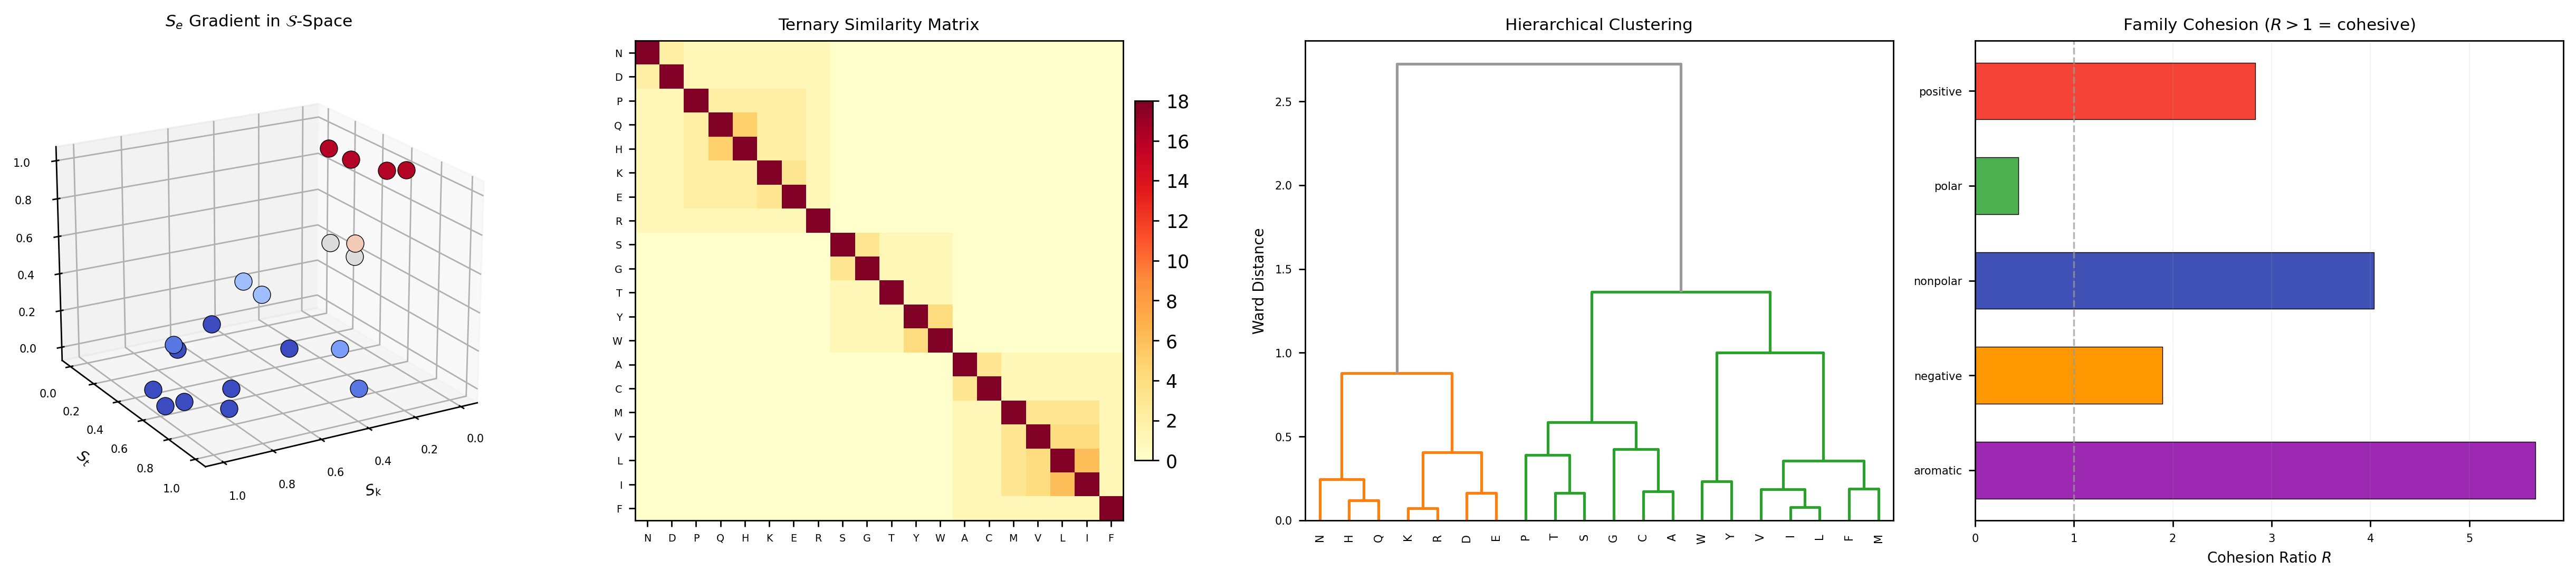
\includegraphics[width=\textwidth]{figures/panel_2_clustering_similarity.png}
    \caption{\textbf{Chemical Family Clustering and Ternary Similarity.}
    (\textbf{A})~Three-dimensional S-entropy space with amino acids coloured by $S_e$ value on a coolwarm gradient (blue = low $S_e$, red = high $S_e$). The electrostatic axis provides the primary separation between nonpolar residues ($S_e = 0$, blue cluster at bottom) and charged residues ($S_e = 1.0$, red cluster at top), with polar residues at intermediate $S_e$ values. This gradient emerges from the physicochemical encoding without any chemical knowledge being imposed.
    (\textbf{B})~Pairwise ternary similarity matrix for all 20 amino acids, sorted by ternary address to place similar residues adjacent. Cell colour encodes shared prefix depth (dark = low similarity, bright = high). The bright diagonal confirms self-identity (depth 18). Off-diagonal bright blocks reveal natural clusters: a nonpolar block (I, V, L, F, M, A), a charged block (D, E, K, R), and aromatic groupings (F, W, Y), all emerging from ternary address proximity.
    (\textbf{C})~Hierarchical clustering dendrogram computed from Euclidean distances in $\mathcal{S}$-space using Ward's method. The tree recovers standard biochemical groupings: charged residues (D, E, K, R, H) form one major clade; nonpolar residues (I, V, L, F, M, A) form another; polar and aromatic residues occupy intermediate branches. No chemical classification was provided to the algorithm.
    (\textbf{D})~Cohesion ratio $R$ (intra-class mean shared prefix depth divided by inter-class mean) for five physicochemical families. $R > 1$ (dashed line) indicates the family is cohesive in ternary space. Aromatic residues show the strongest cohesion ($R = 5.67$), followed by nonpolar ($R = 4.03$), positive ($R = 2.83$), and negative ($R = 1.90$). Polar residues ($R = 0.44$) are non-cohesive, reflecting genuine heterogeneity spanning Cys ($S_k = 0.78$) to Gln ($S_k = 0.11$). Four of five families pass the cohesion test.}
    \label{fig:clustering_similarity}
\end{figure*}

\begin{figure*}[!htbp]
    \centering
    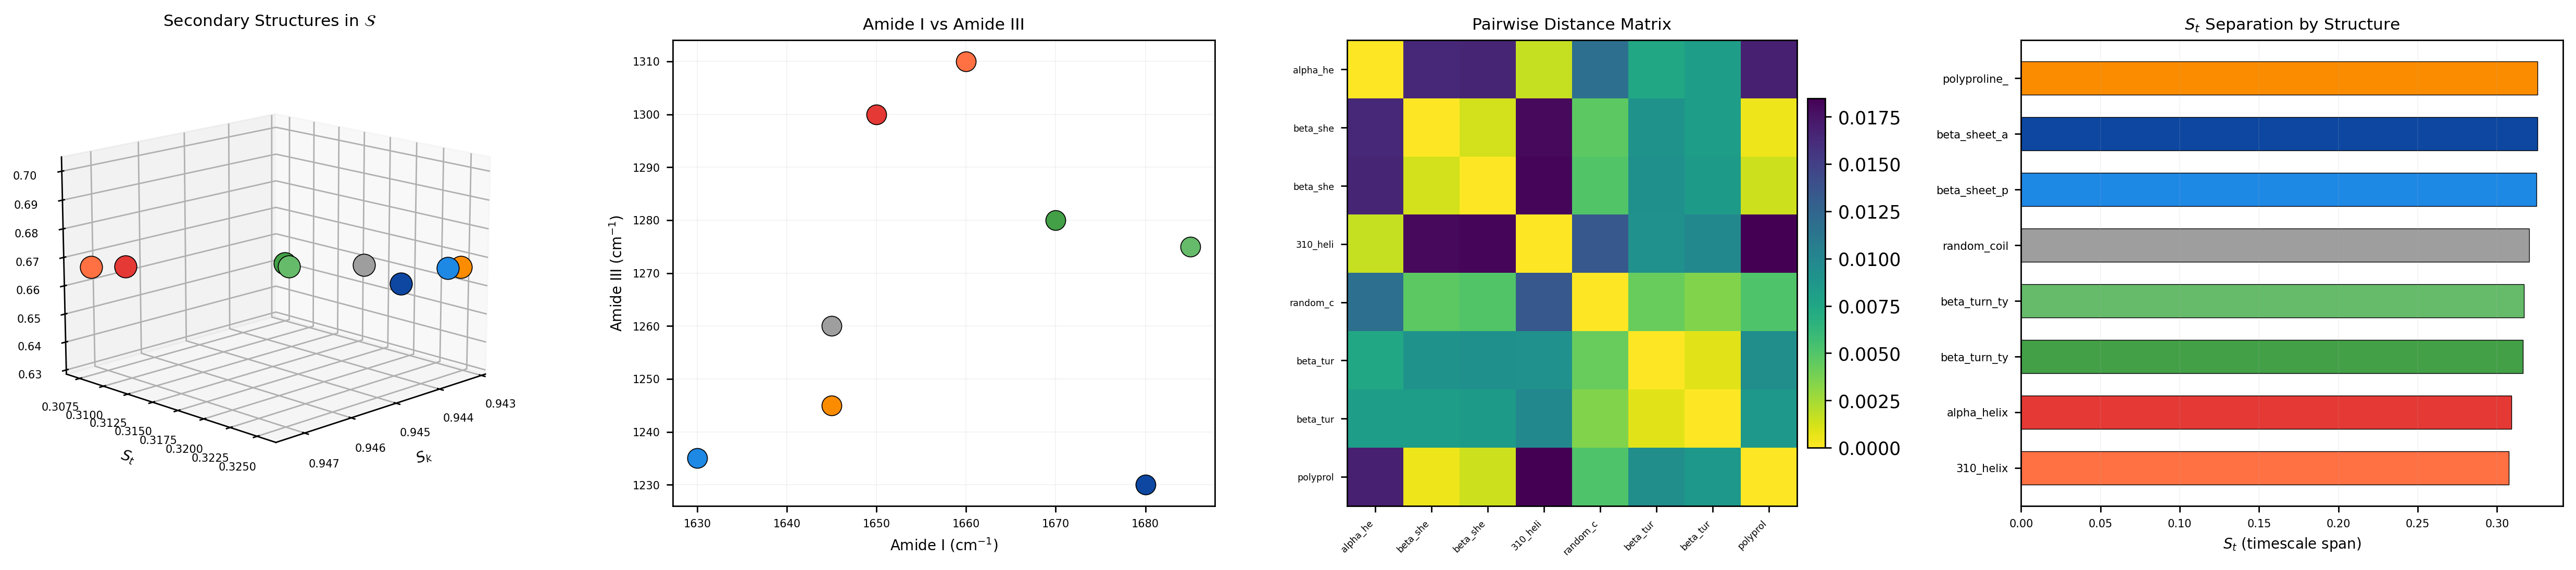
\includegraphics[width=\textwidth]{figures/panel_3_secondary_structure.png}
    \caption{\textbf{Secondary Structure Encoding from Amide Band Frequencies.}
    (\textbf{A})~Eight secondary structure types embedded in S-entropy space, computed from their characteristic amide I, II, III, and A band frequencies. All structures occupy a compact region near $S_k \approx 0.94$, $S_t \approx 0.31$, $S_e \approx 0.67$, reflecting the fact that amide bands are chemically similar backbone vibrations. Separation between structure types is achieved through fine differences in $S_t$ (timescale span), requiring higher trit depths for resolution.
    (\textbf{B})~Amide I versus Amide III frequency scatter plot for all eight structure types. $\alpha$-helix (red) and $\beta$-sheet (blue shades) occupy distinct frequency regions: $\alpha$-helix at amide I $\approx 1650$ cm$^{-1}$, $\beta$-sheet parallel at $\approx 1630$ cm$^{-1}$, $\beta$-sheet antiparallel at $\approx 1680$ cm$^{-1}$. These frequency differences, though small ($\sim 30$--$50$ cm$^{-1}$), are the physical basis for infrared secondary structure determination and map to distinct S-entropy coordinates.
    (\textbf{C})~Pairwise Euclidean distance matrix in $\mathcal{S}$-space. The maximum distance is 0.019 ($\alpha$-helix vs.\ $\beta$-sheet antiparallel); the minimum is 0.0004 ($\beta$-sheet parallel vs.\ polyproline II). The viridis colour scale reveals that $\alpha$-helix and $3_{10}$-helix (warm colours) are most distant from $\beta$-sheet variants (cool colours), consistent with the known spectroscopic distinction between helical and extended conformations.
    (\textbf{D})~$S_t$ coordinate (timescale span) for each secondary structure type, sorted by value. $S_t$ is the primary discriminating coordinate: $3_{10}$-helix has the lowest $S_t$ (narrowest frequency range) while $\beta$-sheet antiparallel and polyproline II have the highest (broadest range due to split amide I band). Full resolution of all eight types is achieved at trit depth 18.}
    \label{fig:secondary_structure}
\end{figure*}

\begin{figure*}[!htbp]
    \centering
    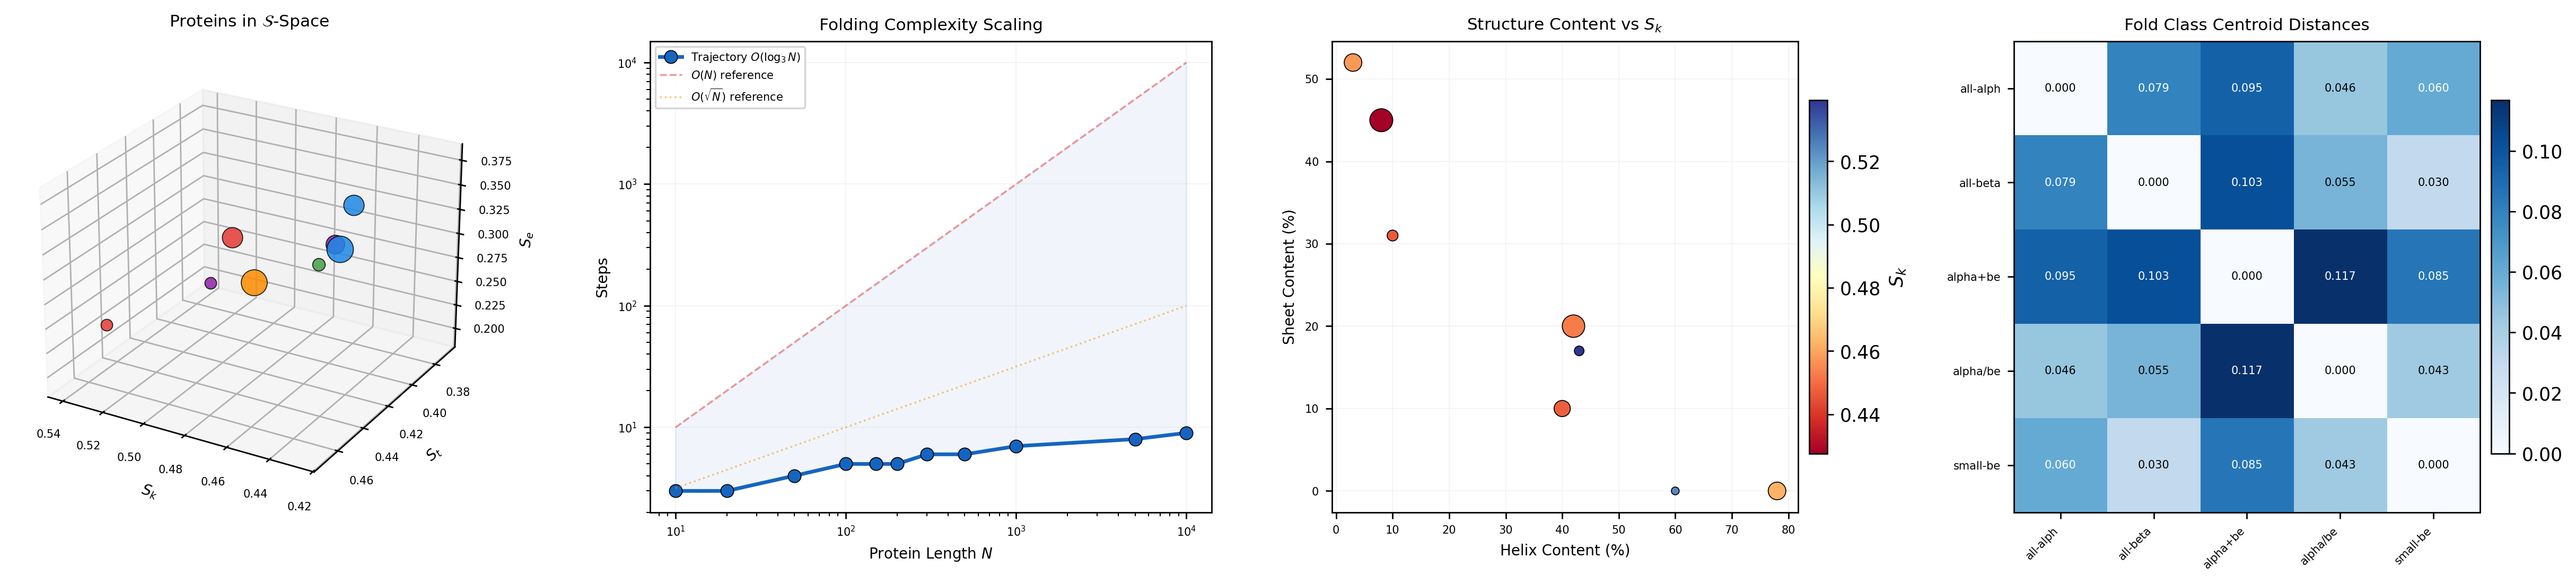
\includegraphics[width=\textwidth]{figures/panel_4_protein_trajectories.png}
    \caption{\textbf{Protein Trajectory Completion and Folding Complexity.}
    (\textbf{A})~Eight test proteins embedded in S-entropy space, coloured by SCOP fold class: all-$\alpha$ (red), all-$\beta$ (blue), $\alpha + \beta$ (purple), $\alpha / \beta$ (orange), small-$\beta$ (green). Point size scales with protein length (30--259 residues). Fold classes occupy distinct regions: all-$\alpha$ proteins (Insulin, Myoglobin) show higher $S_k$ (more hydrophobic composition); all-$\beta$ proteins (SOD1, Carbonic Anhydrase II) show higher $S_e$ (more charged residues). The $\alpha + \beta$ class (Crambin, Lysozyme) occupies an intermediate position with lower $S_e$.
    (\textbf{B})~Folding complexity scaling on log--log axes. Trajectory completion steps (blue circles) grow as $O(\log_3 N)$ with protein length $N$, compared with $O(N)$ (red dashed) and $O(\sqrt{N})$ (orange dotted) references. A 150-residue protein requires 5 trajectory steps; a 10{,}000-residue complex requires only 9. The shaded region represents the complexity reduction from Levinthal's $O(3^N)$ brute-force search. For a 150-residue protein, this corresponds to a reduction from $3^{150} \approx 10^{71}$ conformations to 5 steps---a factor of $\sim 10^{69}$.
    (\textbf{C})~Helix content versus sheet content for the eight test proteins, with point colour encoding $S_k$ (hydrophobicity) and point size encoding protein length. $S_k$ correlates positively with helix content ($r = +0.46$) and negatively with sheet content ($r = -0.48$), consistent with the known preference of hydrophobic residues for $\alpha$-helical packing.
    (\textbf{D})~Fold class centroid distance matrix. Each cell shows the Euclidean distance between fold class centroids in $\mathcal{S}$-space. The largest separation is $\alpha + \beta$ versus $\alpha / \beta$ ($d = 0.117$); the smallest is all-$\beta$ versus small-$\beta$ ($d = 0.030$). The block structure confirms that sequence-level S-entropy coordinates carry structural information sufficient to discriminate major fold classes.}
    \label{fig:protein_trajectories}
\end{figure*}
